\documentclass[uplatex,dvipdfmx,a4paper,12pt]{article}

% フォントを Times New Roman にする
\usepackage{newtxtext,newtxmath}

\usepackage{amsmath,amsthm,amssymb}
\usepackage[dvipdfmx]{graphicx}
\usepackage{bm}
%
\usepackage{multirow}
\usepackage{wrapfig}

\usepackage{caption}
\captionsetup[figure]{format=plain, labelformat=simple, labelsep=period, font=footnotesize}

\usepackage{geometry}
\geometry{left=25truemm, right=25truemm, top=25truemm, bottom=25truemm}

%
\abovecaptionskip=-1pt
%\belowcaptionskip=-1pt
%
\renewcommand{\baselinestretch}{0.96} %全体の行間調整
% \renewcommand{\figurename}{Fig.}
% \renewcommand{\tablename}{Tab.}
%
\makeatletter 
\def\section{\@startsection {section}{1}{\z@}{1.5 ex plus 2ex minus -.2ex}{0.5 ex plus .2ex}{\bf}}
\def\subsection{\@startsection{subsection}{2}{\z@}{0.2\Cvs \@plus.5\Cdp \@minus.2\Cdp}{0.1\Cvs \@plus.3\Cdp}{\reset@font\normalsize\bfseries}}
\makeatother 
% %

\pagestyle{empty}

\graphicspath{{../../figures//}}

\begin{document}

%%%%%%
% はじめに
%%%%%%
\begin{center}
\textbf{Relaxation Behavior of Network Polymers with Random Connectivity}

\vspace{\baselineskip}
Hiroshi sasaki

\vspace{0.5\baselineskip}
Toagosei Co., Ltd.

8 Showa-cho, Minato-ku, Nagoya, Aichi, JAPAN

Phone: +81-52-611-9923 E-mail: hiroshi\_sasaki@mail.toagosei.co.jp
\end{center}

% \vspace{\baselineskip}
\section*{Introduction}

To explain the origin of the high fracture toughness of rubber, Andrews' model, in which crack propagation is suppressed by energy dissipation such as hysteresis loss, has been proposed [1].
As a development from the classical "affine network model" of rubber elasticity, the "phantom network model (PNM)," which focuses on nodal fluctuations, was proposed.
According to Flory, PNM behavior is exhibited in random networks with fluctuations of strands identical to the melt state [2].
We have been investigating the possibility that this nodal fluctuation-derived dissipation could be a viscoelastic energy dissipation model.

We previously reported that PNM can be reproduced by changing the connectivity of a regular structure network to random [3].
Here, we report the results of an MD simulation study of the relaxation behavior of network polymers with random connectivity.

\begin{wrapfigure}[12]{r}[0pt]{0.45\textwidth}
	\centering
	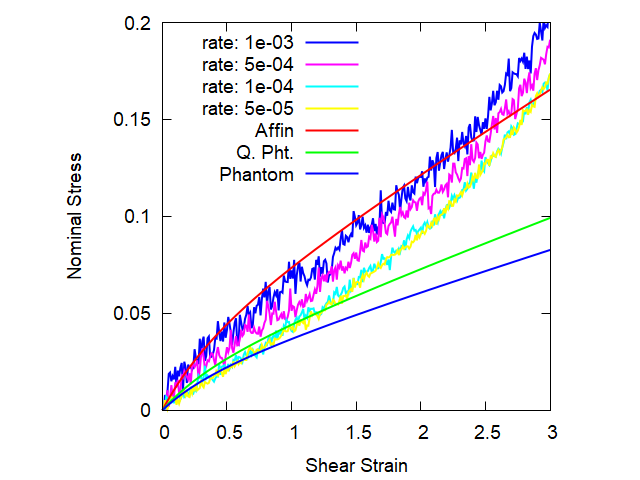
\includegraphics[width=.45\textwidth]{Shear_Random_4chain_N20.png}
    \vspace{2mm}
    \caption{SS Curves for 4-chain NW of KG Strands(N=40)}
    \label{fig:deform}

    \vspace{3mm}
    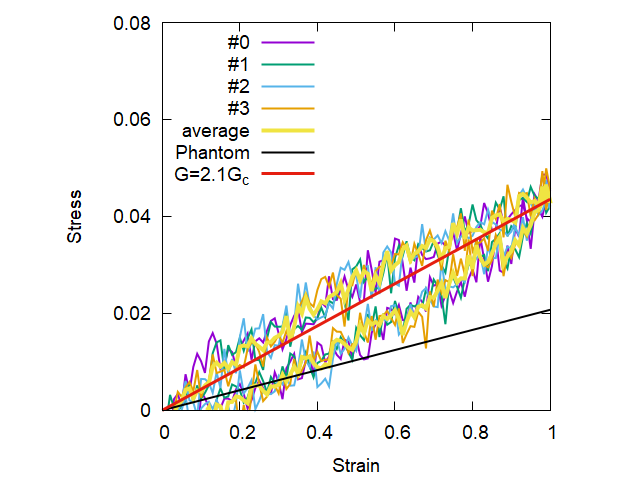
\includegraphics[width=.45\textwidth]{CyclicDeform_4chain_rate_2e-4.png}
    \vspace{2mm}
    \caption{Hysteresis Curves for 4-chain NW (N=40) by Cyclic Shear ($\lambda = 1$)}
    \label{fig:hyst}
\end{wrapfigure}

\section*{Results and Discussion}

(Simulation) 

A network of 3-, 4- and 6-branches with random connectivity was created according to a previous report [3].
As network strands, we used KG strands with LJ interactions introduced between segments and phantom strands without interactions.
Its behavior at equilibrium and during deformation, uniaxial elongation or shear, was evaluated by molecular dynamics simulations using the COGNAC simulator on OCTA.

(Evaluation of mechanical response) 

When phantom chains with no inter-segmental interactions were used, the response was similar to that of the theoretical phantom network. 
% due to the reduction in shear rate.
For KG chains, the modulus of elasticity was about twice that of the PNM model, G, at shear rates where the deformation rate dependence disappears.

% \begin{wrapfigure}{r}[0pt]{0.45\textwidth}
% 	\centering
% 	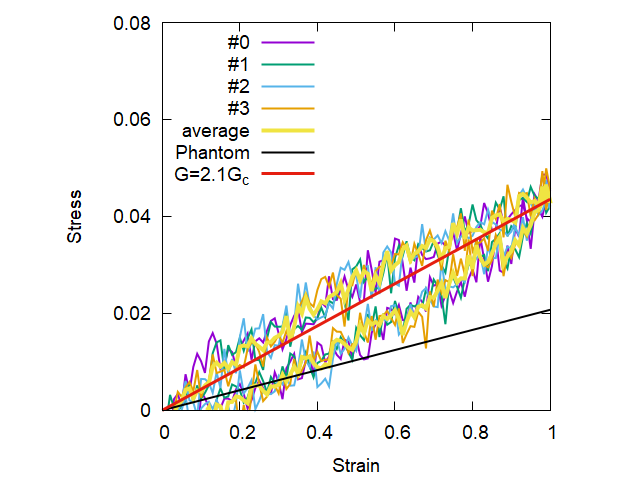
\includegraphics[width=.45\textwidth]{CyclicDeform_4chain_rate_2e-4.png}
%     \vspace{2mm}
%     \caption{Hysteresis Curves for 4-chain NW by Cyclic Shear ($\lambda = 1$)}
%     \label{fig:hyst}
% \end{wrapfigure}

(Hysteresis)

The difference in elastic modulus was estimated to be due to both intersegmental interaction and entanglement.
The difference in elastic modulus was estimated to be due to both intersegmental interaction and entanglement.

% \begin{figure}[hb]
%     \begin{minipage}{0.45\hsize}
%         \begin{center}
%         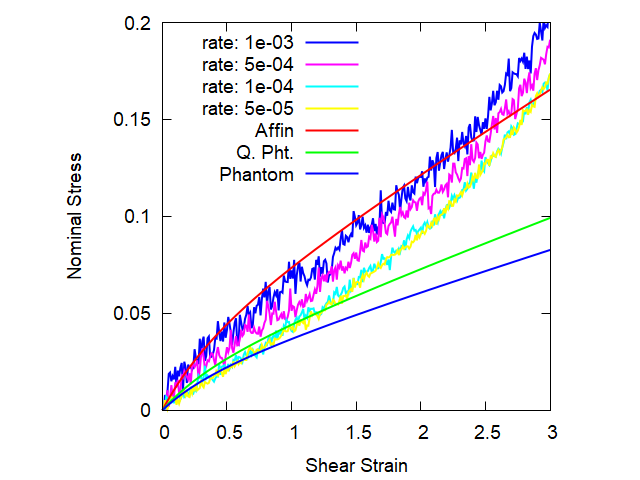
\includegraphics[width=\textwidth]{Shear_Random_4chain_N20.png}
%         \vspace{1mm}
%         \caption{SS Curves for 4-chain NW of \\Phantom Strands}
%         \label{fig:deform}
%         \end{center}
%     \end{minipage}
%     \begin{minipage}{0.1\hsize}
%     \end{minipage}
%     \begin{minipage}{0.45\hsize}
%         \begin{center}
%         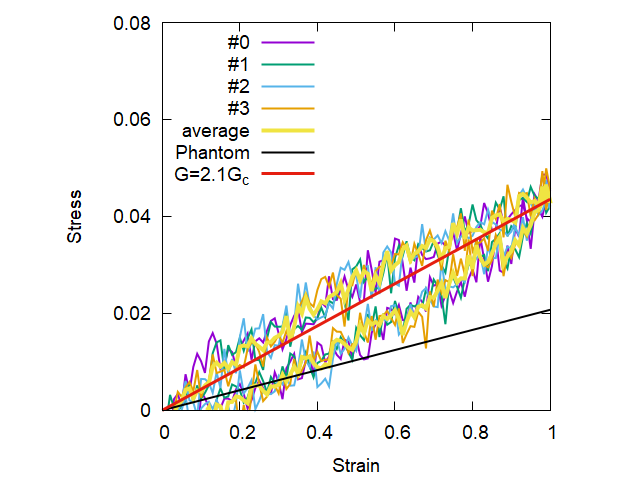
\includegraphics[width=\textwidth]{CyclicDeform_4chain_rate_2e-4.png}
%         \vspace{1mm}
%         \caption{Hysteresis Curves for 4-chain NW by Cyclic Shear ($\lambda = 1$)}
%         \label{fig:hyst}
%         \end{center}
%     \end{minipage}
%     \begin{minipage}{0.33\hsize}
%         \begin{center}
%         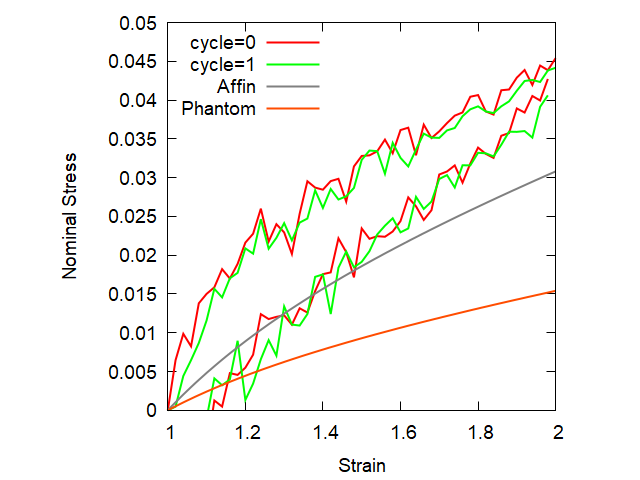
\includegraphics[width=\textwidth]{hyst_4Chain.png}
%         \vspace{1mm}
%         \caption{Strand Exchange Procedure}
%         \label{fig:exc}
%         \end{center}
%     \end{minipage}
% \end{figure}

% \vspace{-7mm}
\begin{thebibliography}{99}
    \small % フォントサイズを下げる
    \setlength{\itemsep}{-2pt} % 行間を縮める
    \bibitem{andrews} E. H. Andrews, Y. Fukahori Journal of Materials Science, 12, 1307 (1977)
    \bibitem{flory} P. J. Flory Proceedings of the Royal Society of London. Series A, 351, 351 (1976)
    \bibitem{sasaki} H. Sasaki, 69th Rheology Symposium Preprint (2021)
\end{thebibliography}

\end{document}